% !TEX root = main.tex
\section{Construction of vFHE}
\begin{frame}{Circuit Description}
	Let $L \in \NN$ and $q_0, \dots, q_L$ be primes. Let $Q^{(k)} = \prod_{i = 0}^k q_i$.
	
	Fresh ciphertexts are defined over $R_{Q^{(L)}}$. The circuit is defined as
	\begin{equation*}
		C_0(\dots(M_{L-1}(C_{L-1}(M_L(C_L(\cdot))))))
	\end{equation*}
	where 
	\begin{itemize}
		\item $C_k$ is evaluation circuit for a single multiplication depth, and
		\item $M_k$ is for relinearization and modulus switchings.
	\end{itemize}
\end{frame}

\begin{frame}{Construction Idea}
	\begin{figure}
		\centering
		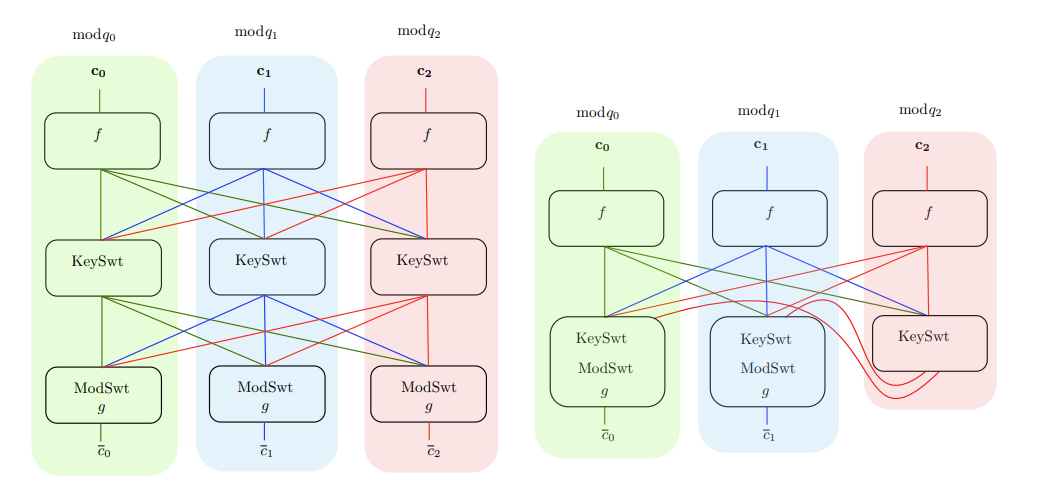
\includegraphics[width=1.1\linewidth]{proofidea}
		\caption{Construction idea (Figure 3 in \cite{CIC:ABPS24}).}
		\label{fig:proofidea}
	\end{figure}
	
\end{frame}